\chapter{Apéndice: diseño de redes neuronales} \label{chapter:appendixA}
\begin{definition}[Normalización por lotes (\textit{Batch normalization})]
    Sea \( \mathcal{B} = (x_{i})_{i=1}^m \) con \( x_{i} \in \real{n} \) un minilote con media \( \widehat{\mu}_\mathcal{B} \) y desviación estándar  \( \widehat{\sigma}_\mathcal{B} \). Sean \( \gamma, \beta \in \real{n} \).

    Definimos la normalización por lotes como la capa que computa la función \( \BN: \real{n} \to \real{n} \):
    \[
        \BN(x; \gamma, \beta) = \gamma \odot \frac{x - \widehat{\mu}_\mathcal{B}}{\widehat{\sigma}_\mathcal{B}} + \beta
    \]
\end{definition}

La normalización por lotes funciona bien cuando el tamaño de cada minilote es suficientemente grande como para que los estimadores \( \widehat{\mu}_\mathcal{B}, \widehat{\sigma}_\mathcal{B} \) sean próximos al valor poblacional (lo que requiere, por lo general, un tamaño de minilote de entre 50 y 100 elementos \cite{luo2018towards}).

\begin{figure}[tb]
    \centering
    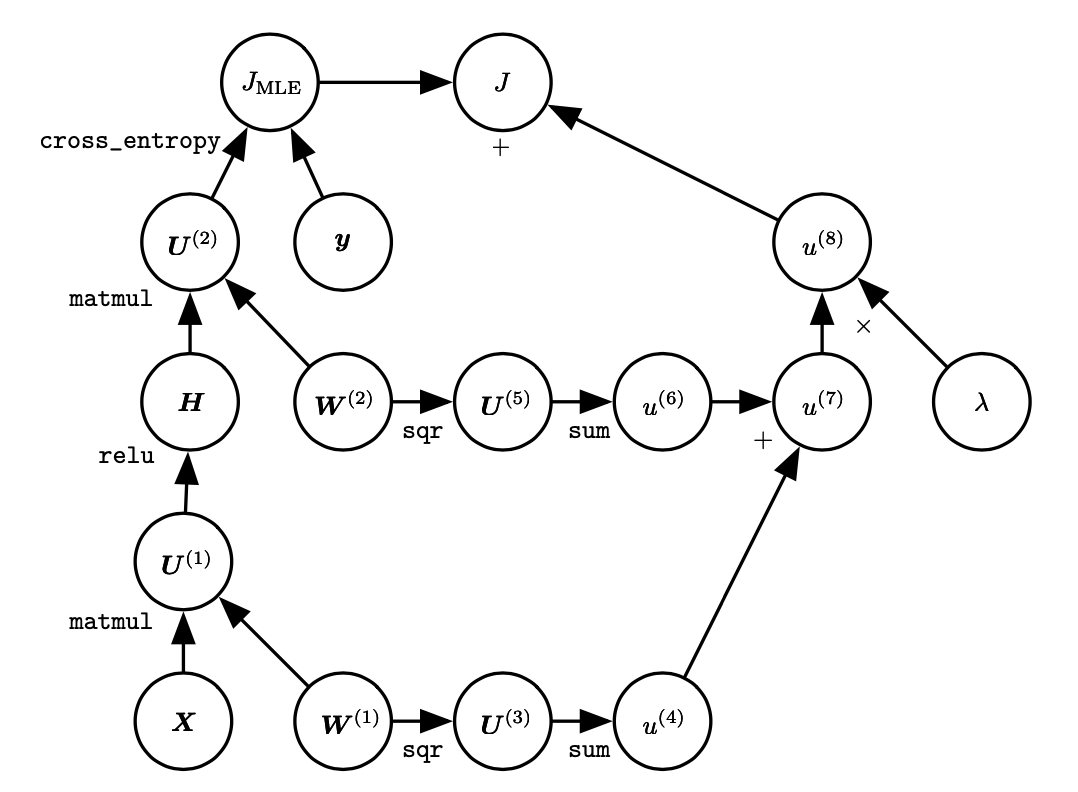
\includegraphics[scale=0.6]{figures/chapter2/grafo.png}
    \caption{Ejemplo de grafo computacional de una red sencilla. El grafo se construye durante la propagación hacia delante en el sentido de las aristas y el gradiente se calcula durante la propagación hacia atrás en sentido inverso, comenzando por la pérdida (nodo \( J\)) \cite{goodfellow2016deep}}
    \label{fig:graph}
\end{figure}


\begin{figure}[tb]
    \centering
    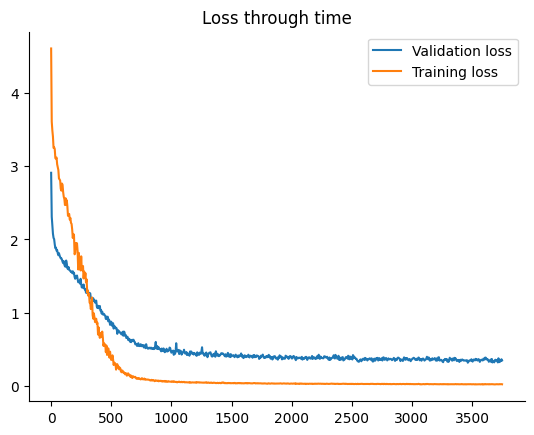
\includegraphics[scale=0.5]{figures/chapter5/loss_big.png}
    \caption{Pérdida sobre el conjunto de entrenamiento y validación a lo largo del entrenamiento. Los valores no son comparables con los de la \cref{fig:loss}, pues la división en símbolos se hace ahora a nivel de palabra, no de caracter. }
    \label{fig:loss_big}
\end{figure}
\begin{figure}[tb]
    \centering
    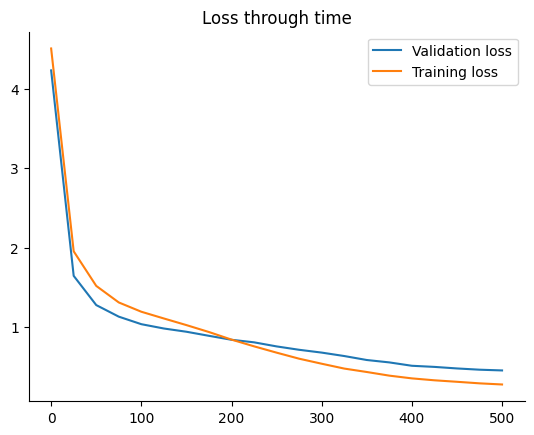
\includegraphics[scale=0.5]{figures/chapter5/loss.png}
    \caption{Gráfica de entrenamiento del modelo, mostrando la pérdida sobre el conjunto de entrenamiento y validación}
    \label{fig:loss}
\end{figure}

\begin{figure}
    \centering
    \begin{subfigure}
        \centering
        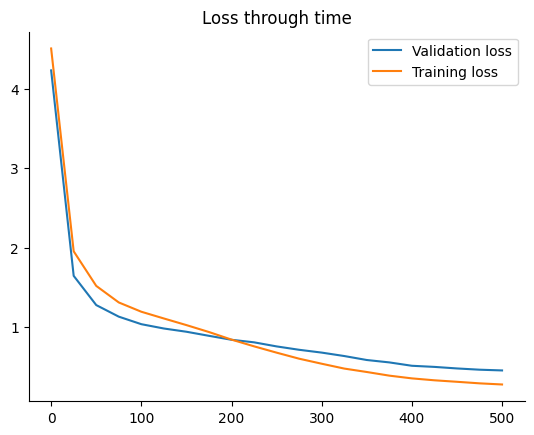
\includegraphics[scale=0.5]{figures/chapter5/loss.png}
        \caption{Gráfica de entrenamiento del modelo, mostrando la pérdida sobre el conjunto de entrenamiento y validación}
        \label{fig:loss}
    \end{subfigure}
    \begin{subfigure}
        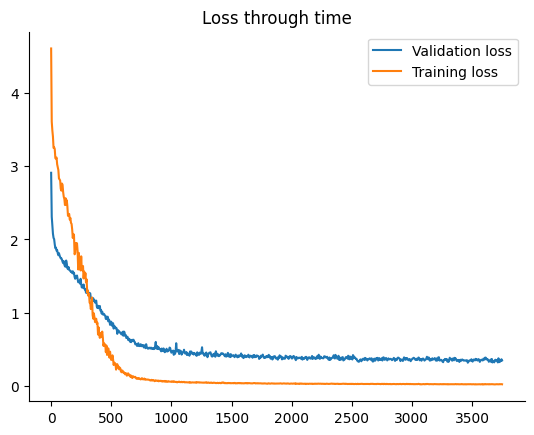
\includegraphics[scale=0.5]{figures/chapter5/loss_big.png}
        \caption{Pérdida sobre el conjunto de entrenamiento y validación a lo largo del entrenamiento. Los valores no son comparables con los de la \cref{fig:loss}, pues la división en símbolos se hace ahora a nivel de palabra, no de caracter. }
        \label{fig:loss_big}
    \end{subfigure}
\end{figure}

\begin{figure}[tb]
    \centering
    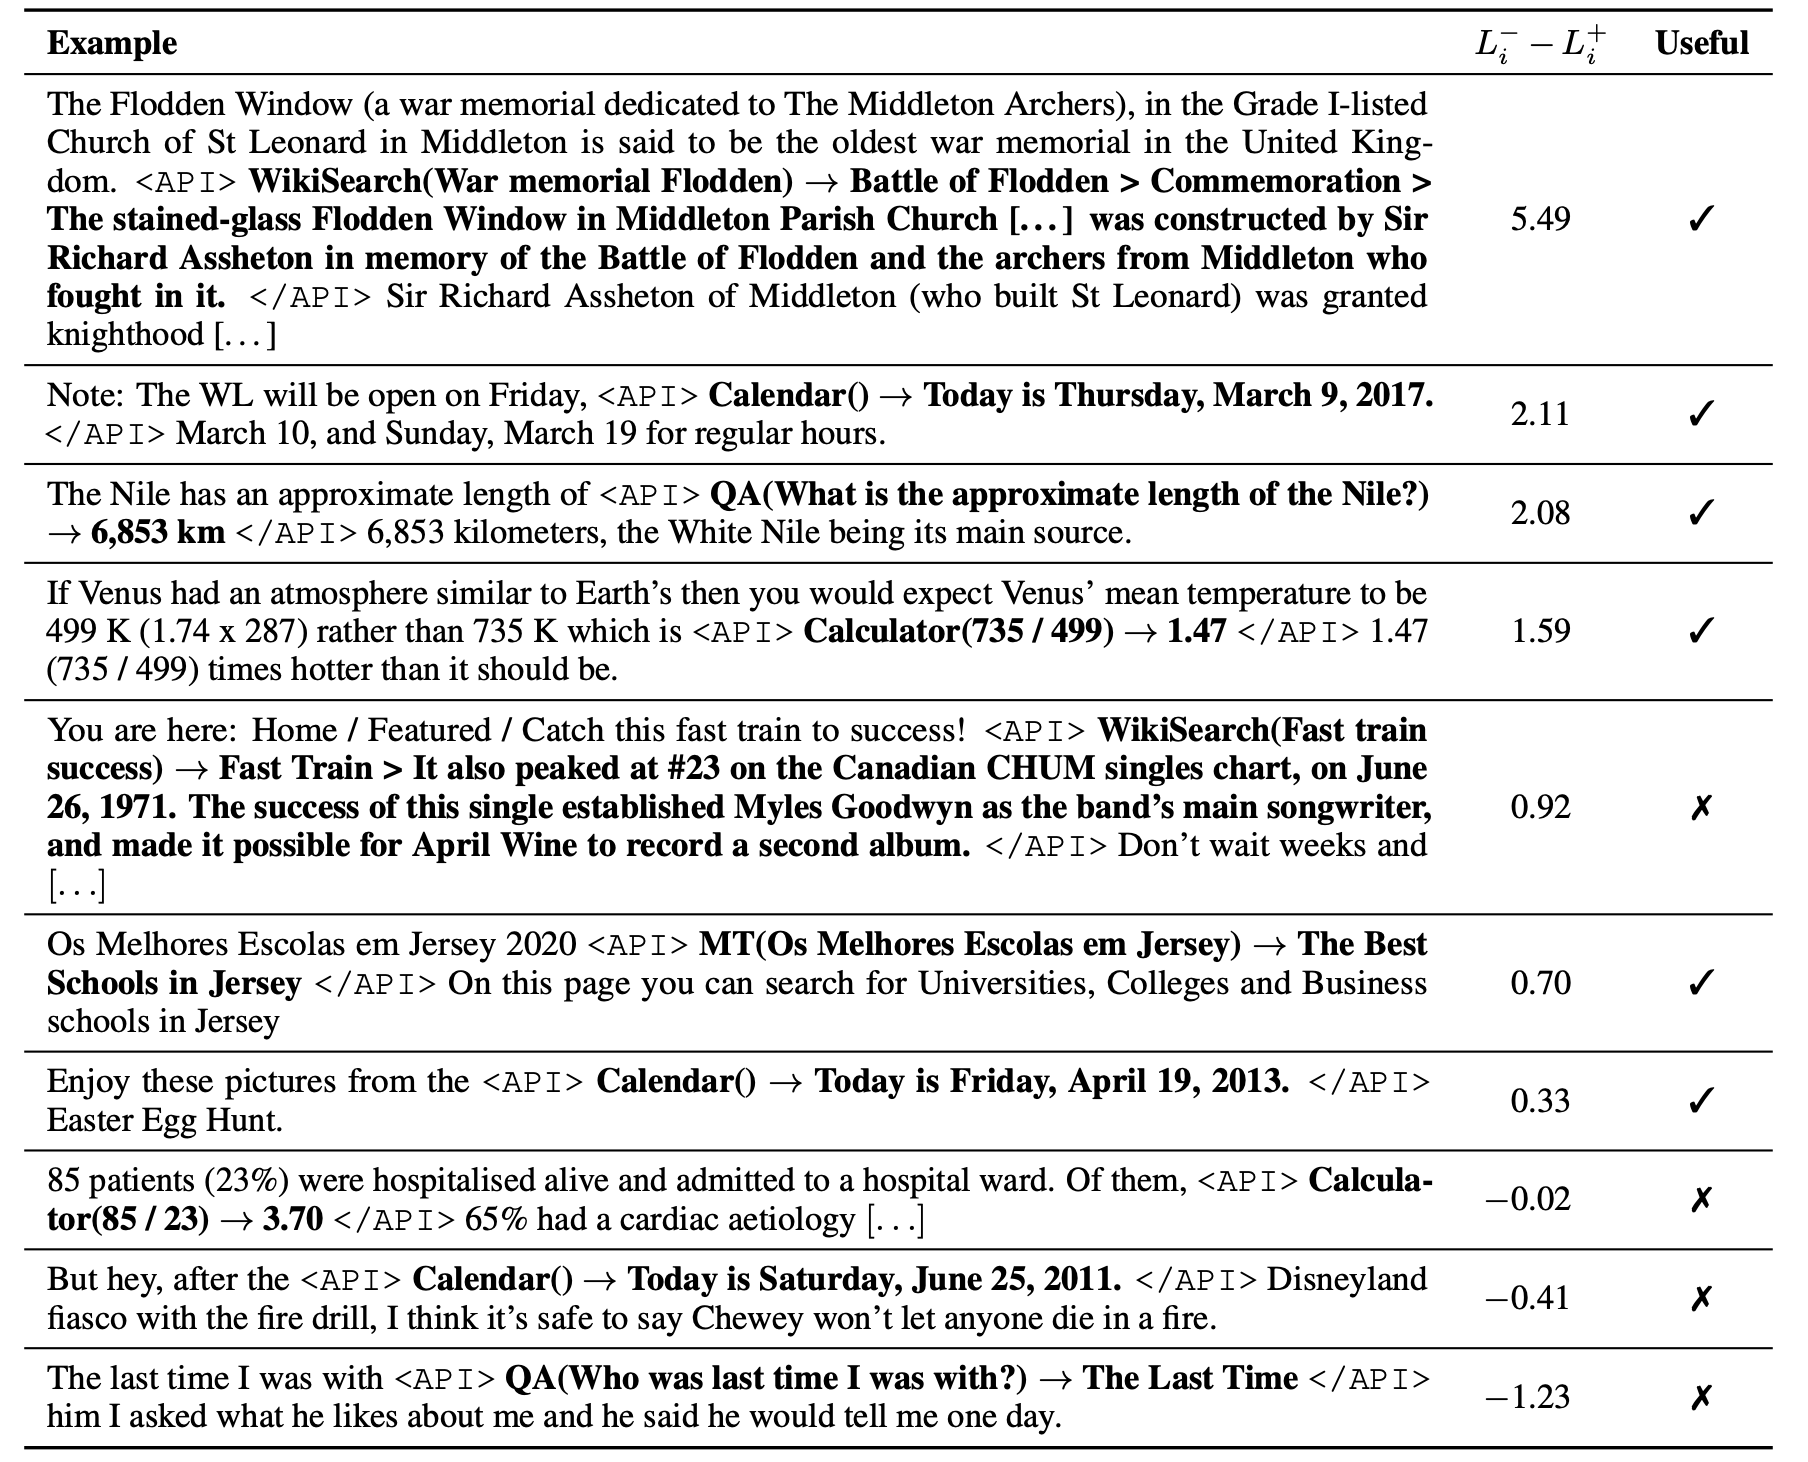
\includegraphics[width=\textwidth]{figures/chapter3/toolformer.png}
    \caption{Ejemplo de llamadas a la API introducidas en la base de datos \cite{schick2023toolformer}. La columna \(L_i^- - L_i^+ \) contiene la diferencia en la evaluación según la entropía cruzada de la respuesta dada por el modelo antes y después de introducir la llamada a la API. \cite{schick2023toolformer}}
    \label{fig:toolformer}
\end{figure}

\begin{figure}[tb]
    \centering
    \begin{subfigure}[b]{0.49\textwidth}
        \centering
        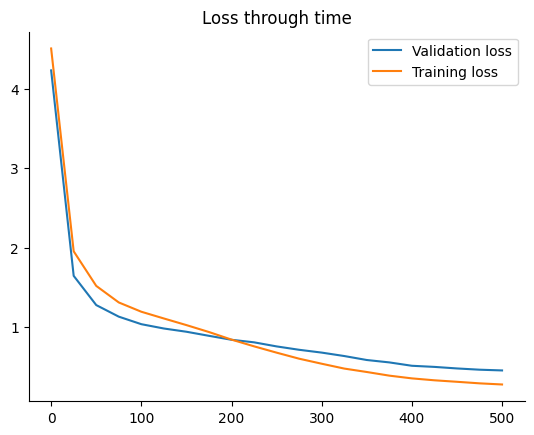
\includegraphics[width=\textwidth]{figures/chapter5/loss.png}
        \caption{Entrenamiento de GPT-1}
        \label{fig:loss}
    \end{subfigure}
    \begin{subfigure}[b]{0.49\textwidth}
        \centering
        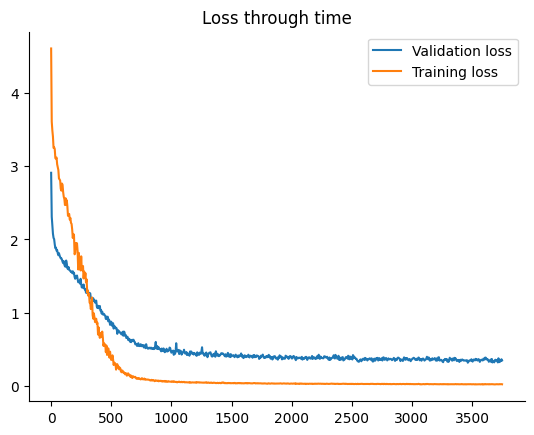
\includegraphics[width=\textwidth]{figures/chapter5/loss_big.png}
        \caption{Entrenamiento de GPT-1}
        \label{fig:loss_big}
    \end{subfigure}
    \caption{Pérdida sobre el conjunto de entrenamiento y validación a lo largo del entrenamiento.}
\end{figure}

\chapter{El estimador de Nadaraya-Watson}
Presentamos a continuación un ejemplo del mecanismo de atención aplicada a problemas de regresión: el estimador de Nadaraya-Watson \cite{watson1964smooth, nadaraya1964estimating}.

Nos encontramos en el marco habitual de un problema de regresión: disponemos de un conjunto de características observadas \( \Set{x_{n}}_{n = 1}^N \) con \( x_{n}  \in \real{n} \) y de un vector \( y = (y_1, \dots, y_N) \) que recoge el valor de la variable objetivo para cada una de las observaciones. Dada una nueva observación \( x_{0} \), queremos aproximar el valor de la variable objetivo \( y_{0} \) mediante un estimador \( \widehat{y}_{0} \).

Definimos la base de datos \( \mathcal{D} = \left\{ (x_{i}, y_{i}) : i = 1, \dots, N \right\} \). Consideramos una función \( \alpha \) normalizada entre \( 0 \) y \( 1 \), esto es:
\[
    \alpha(q, k_{i}) = \frac{a(q, k_{i})}{\sum_j \alpha(q, k_{j}) }
\]
para alguna función \( a : \real{n} \times \real{n} \to \realo \). La atención de \( q \) sobre \( \mathcal{D} \) es:
\[
    \attention(q, \mathcal{D}; \alpha) = \sum_i  \alpha(q, k_{i}) v_{i} = \sum_i \frac{a(q, k_{i})}{\sum_j \alpha(q, k_{j})} v_{i}
\]

Podemos ahora aproximar \( y_{0} \) mediante el estimador 
\begin{equation}\label{eq:kde}
    \widehat{y}_{0} = \left\langle y, \attention(x_{0}, \mathcal{D}; \alpha) \right\rangle
\end{equation}

La \cref{fig:regression} muestra el resultado de estimar la distribución de \( n = 100 \) puntos de la forma \( (x_{i}, y_{i}) \) siendo \( (x_{i}) \) una sucesión ordenada de puntos en \( [0, 5] \), \( y_{i} = x_{i} + \sin(x_{i}) + \epsilon \) con \( \epsilon \sim \mathcal{N}(0, 1) \). Para ello, utilizamos una partición equiespaciada \( x^\text{val}_{i} \) de \( [0, 5] \) con 100 puntos y estimamos \( \widehat{y}^\text{val} \) usando la \cref{eq:kde} con varios \textit{kernel} de similitud distintos:
\[
    \begin{split}\begin{aligned}
    a(q, k) & = \exp\left(-\frac{1}{2} \|q - k\|^2 \right) && \mathrm{Gaussiana} \\
    a(q, k) & = \begin{cases}
        1 &\text{ si } \|q - k\| \leq 1 \\
        0 &\text{ si no}
    \end{cases} && \mathrm{Boxcar}
    \\
    a(q, k) & = \max\left(0, 1 - \|q - k\|\right) && \mathrm{Epanechikov}
    \end{aligned}\end{split}
\]

La estimación es notablemente precisa, aunque la suavidad de la estimación depende del tipo concreto de \textit{kernel} escogido. La \cref{fig:kernel} muestra una visualización de los pesos de atención: observamos que las magnitudes mayores se concentran en torno a la diagonal, dado que \( x^\text{val}_{i} \simeq x^j \) para índices \( i, j \) cercanos. 

\begin{figure}[tb]
    \centering
    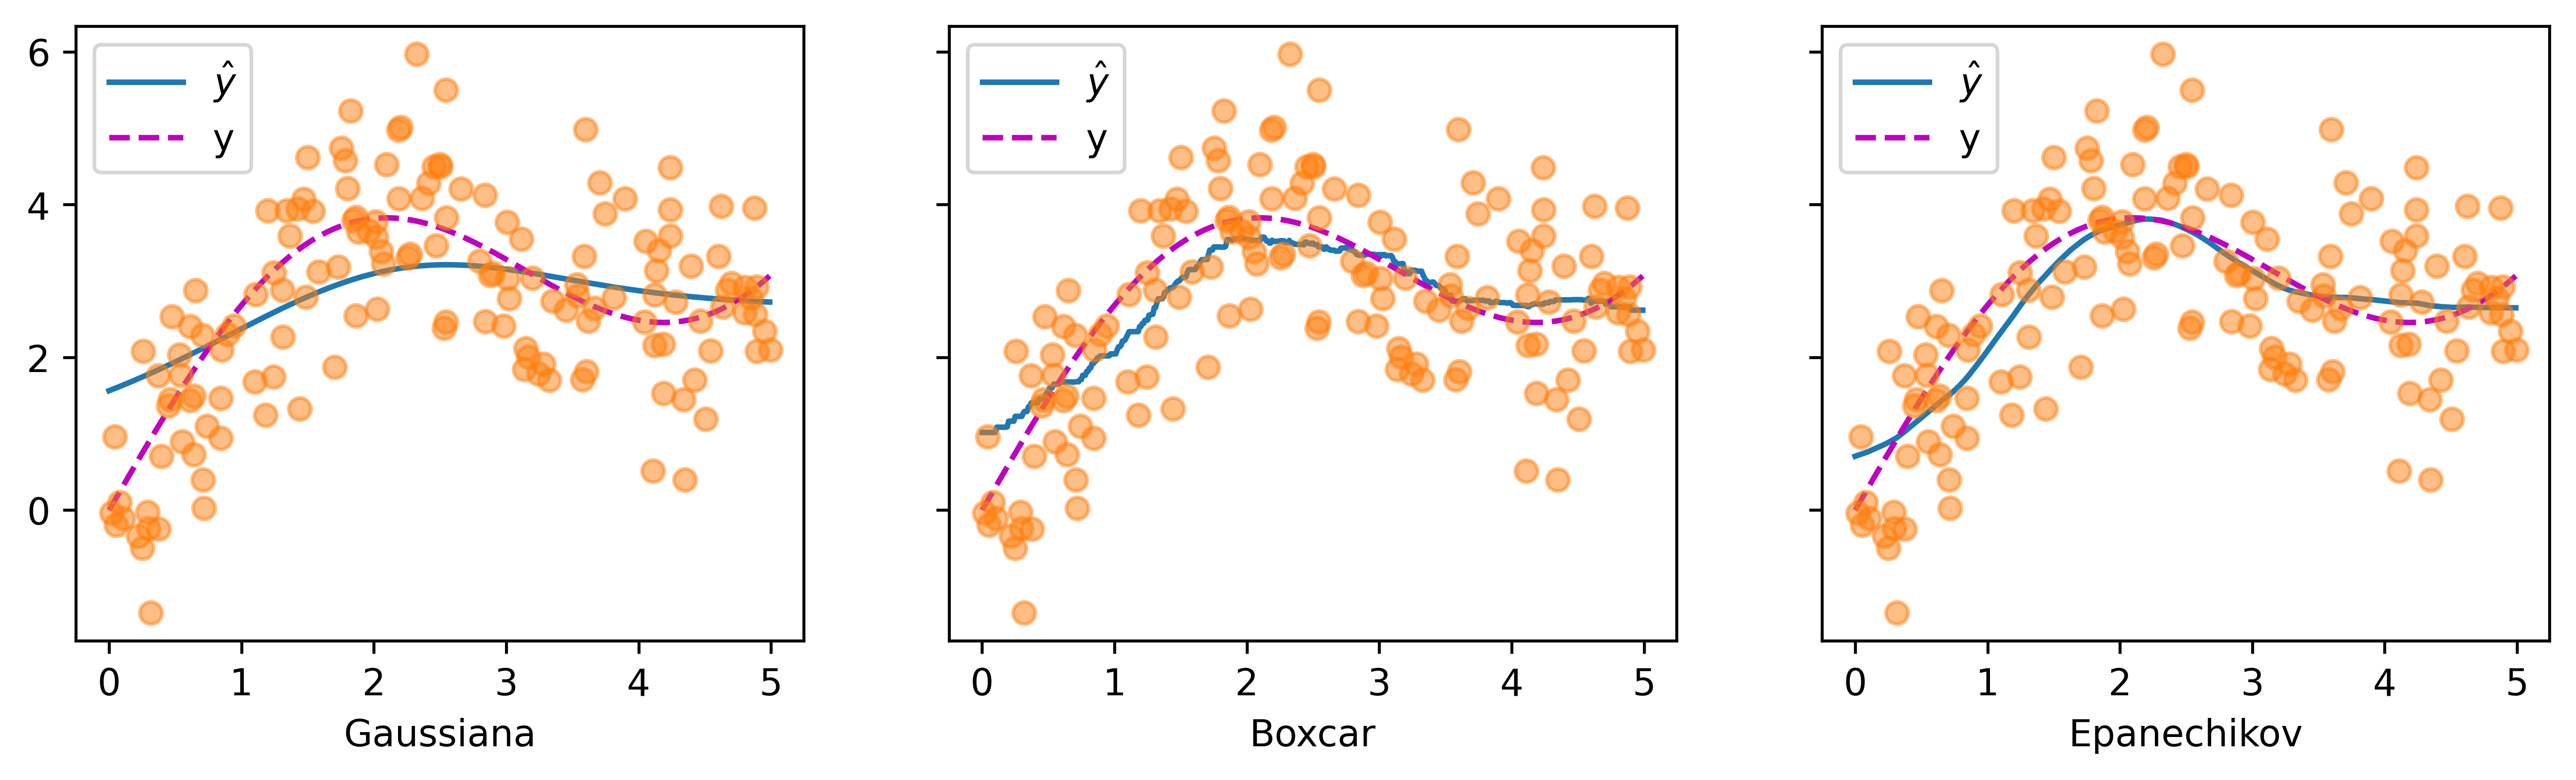
\includegraphics[width=\textwidth]{figures/chapter4/regression.png}
    \caption{Estimación de la función \( y \) mediante la estimación del valor de la variable objetivo sobre una partición equiespaciada del intervalo \( [0, 5] \) usando tres kérneles de similitud distintos.}
    \label{fig:regression}
\end{figure}

Esta forma de utilizar la atención es una forma de \textit{estimación de densidad de kernel}, una técnica clásica de inferencia no paramétrica que tiene la ventaja de que no requiere de ningún entrenamiento. Existen diversas heurísticas para elegir el \textit{kernel} \cite{silverman1986density} y puede probarse que si la anchura del \textit{kernel} se ajusta adecuadamente conforme se añaden observaciones entonces el método converge al valor real \( \E \llbracket y | x = x \rrbracket \) \cite{mack1982weak}.

\begin{figure}[tb]
    \centering
    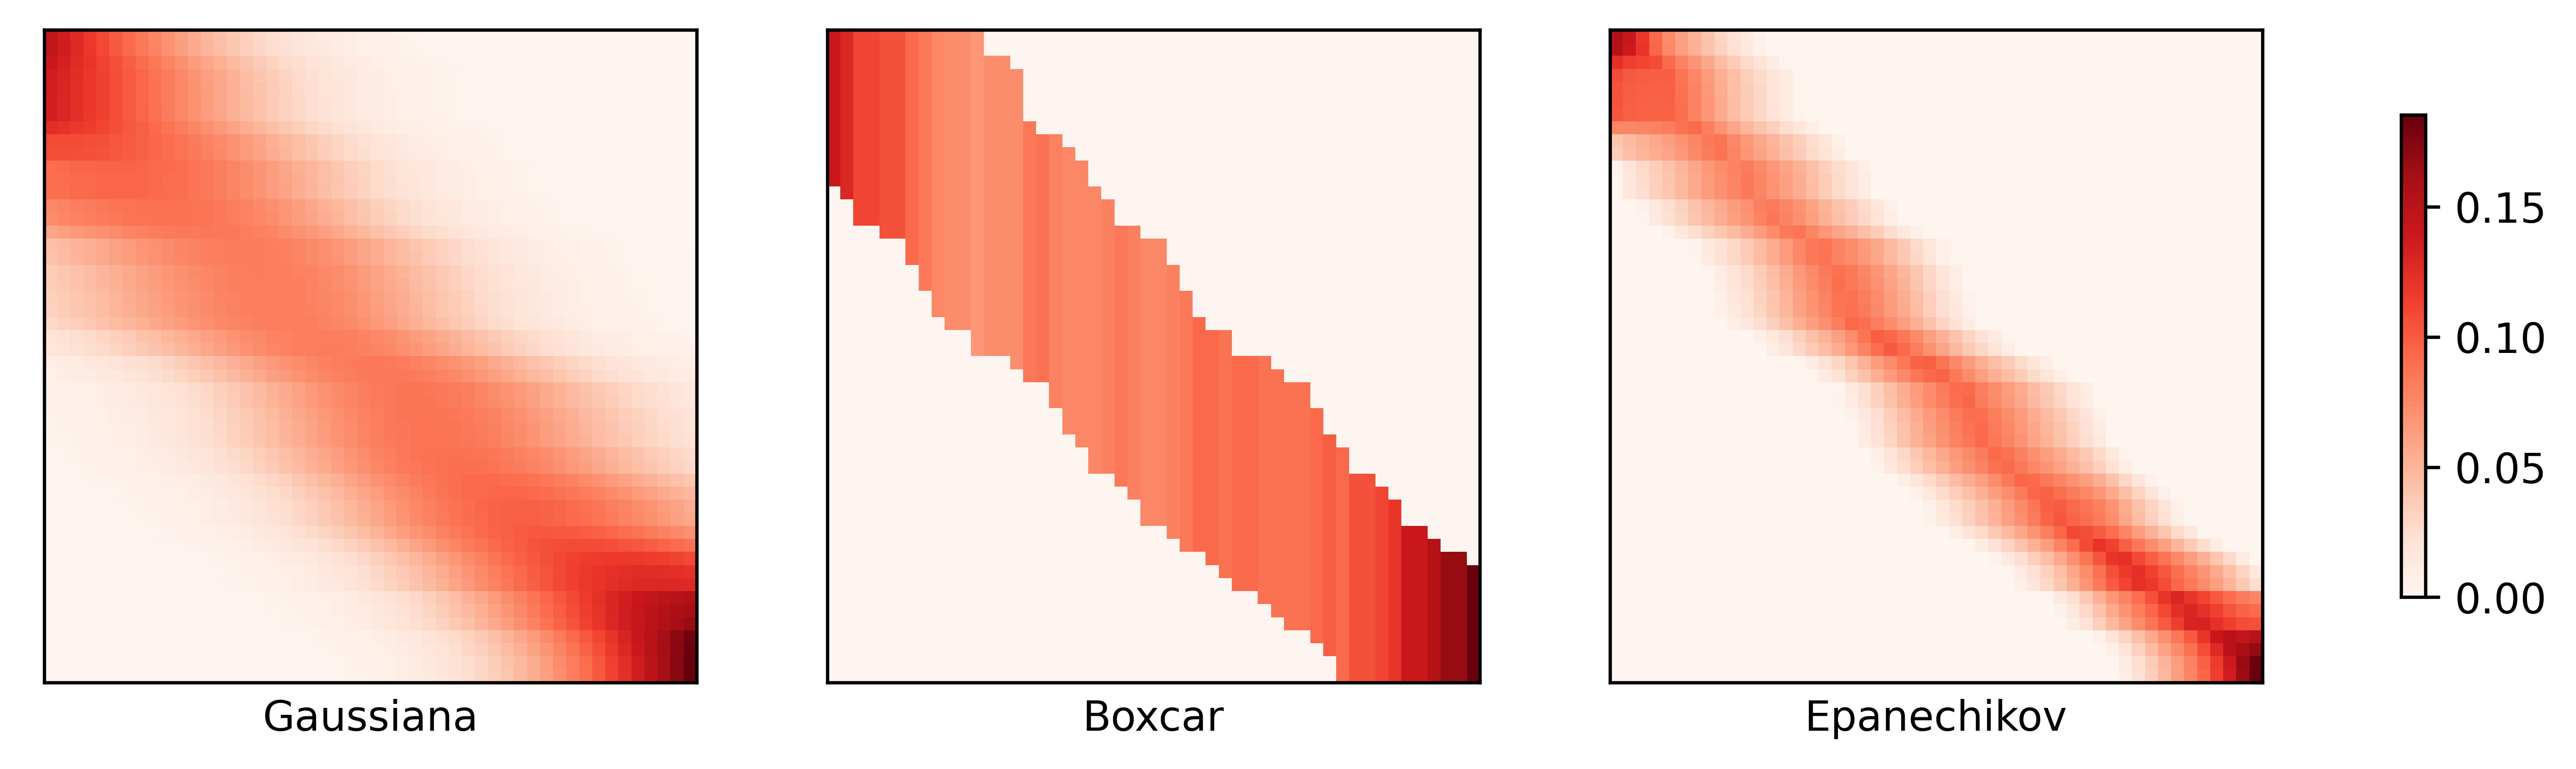
\includegraphics[width=\textwidth]{figures/chapter4/kernel.png}
    \caption{Visualización de los pesos de atención. Cada fila representa uno de los puntos aproximados y cada columna una componente del vector de atención. El color representa la magnitud de la componente.}
    \label{fig:kernel}
\end{figure}

El estudio del estimador de Nadaraya-Watson cumple un triple propósito: en primer lugar, muestra la flexibilidad de los métodos de atención y su relación con métodos clásicos de inferencia estadística. En segundo lugar, sirve para exhibir una de los grandes atributos de los métodos de atención: la posibilidad de visualizar los pesos de atención a fin de poder entender el funcionamiento del modelo. En tercer lugar, muestra lo decisivo de realizar una buena elección de la representación de la base de datos (claves y valores). En última instancia, la complejidad de elegir representaciones adecuadas lleva a diseñar esta representación de forma que sea \textit{aprendida} como una parte más de los parámetros del modelo.
